\subsubsection{Wurfmechanismus}
\begin{figure}[h!]
	\centering
	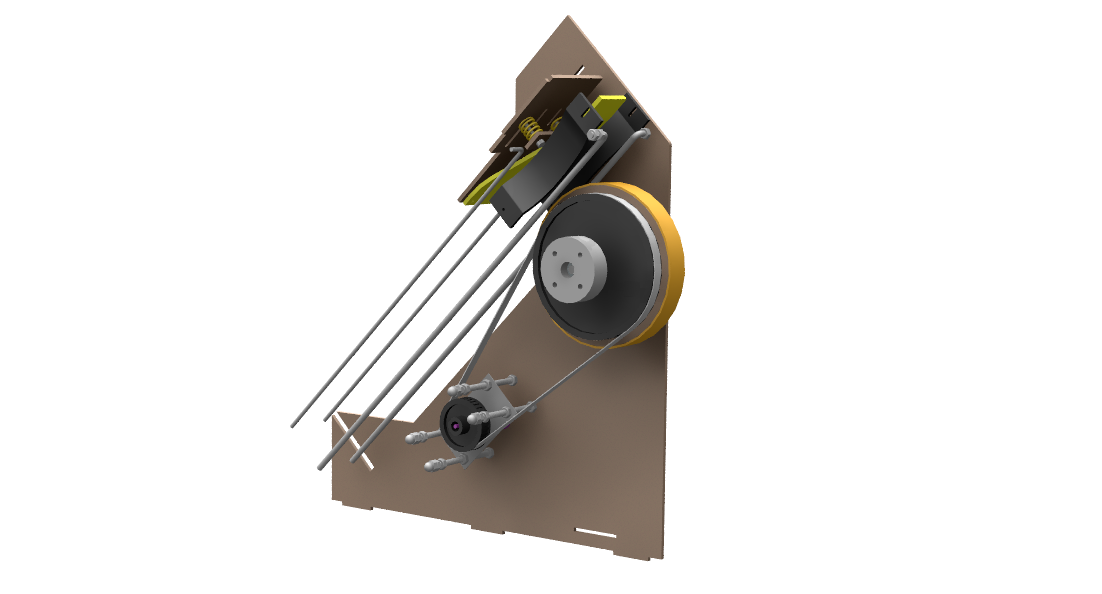
\includegraphics[width=\linewidth]{../../fig/Wurfmechanismus}
	\caption{Wurfmechanismus}
	\label{fig:Wurfmechanismus}
\end{figure}
\paragraph{Komponentenbeschrieb}

Hauptstück des Wurfmechanismus ist das Wurfrad, welches durch Drehung um seine eigene Achse die Bälle beschleunigt.
Das aus fünf MDF-Tellern bestehende Wurfrad ist auf einer  Aluminium-Achse montiert. Die Achse ist mit zwei an seinen Enden angebrachten Radiallagern mit den Seitenwänden des Drehturmes verbunden. Auf der Achse befindet sich weiter ein Zahnriemenrad, welches über einen Zahnriemen die Verbindung zum antreibenden BLDC-Motor ermöglicht.
Um die Reibung zwischen den Bällen und dem Wurfrad zu erhöhen wurde ein Gummiband auf das Rad geklebt.

\paragraph{Entwicklungsprozess}

Da der Wurfmechanismus die zentrale Einheit der Maschine darstellt, wurde ein spezielles Augenmerk auf ihn gerichtet. Würde er nicht funktionieren, wäre die gesamte Konstruktion untauglich. Nach diversen mehr oder weniger sinnvollen Lösungsansätzen, entschied man sich daher für eine der konservativeren Bauarten.
Das Wurfrad als beschleunigendes Element hat sich bei vielen anderen Tennisball-Wurfmaschinen bewährt und bot sich daher als sichere Lösung an.
Zu Beginn des Entwicklungsprozesses hielt man es für die beste Lösung ein Rad aus dem Modellbau zu kaufen. Man entschied sich später allerdings, das komplette Wurfrad selber herzustellen. Mit dieser Lösung, war es möglich, das Rad besser in die Konstruktion einzupassen. Ausserdem konnte es zusammen mit den anderen zu lasernden Komponenten gefertigt werden, was nur wenig Mehraufwand bedeutete.